\tikzset{basic/.style={draw,fill=blue!50!green!20,
                       text badly centered,minimum width=3em}}
\tikzset{input/.style={basic,circle}}
\tikzset{weights/.style={basic,rectangle,minimum width=2em}}
\tikzset{functions/.style={basic,circle,fill=blue!50!green!20}}
\newcommand{\addsymbol}{\draw[thick] (0.5em,0.5em) -- (0,0.5em) -- 
                        (0,-0.5em) --  (-0.5em,-0.5em)
                        (0em,0.75em) -- (0em,-0.75em)
                        (0.75em,0em) -- (-0.75em,0em);}

    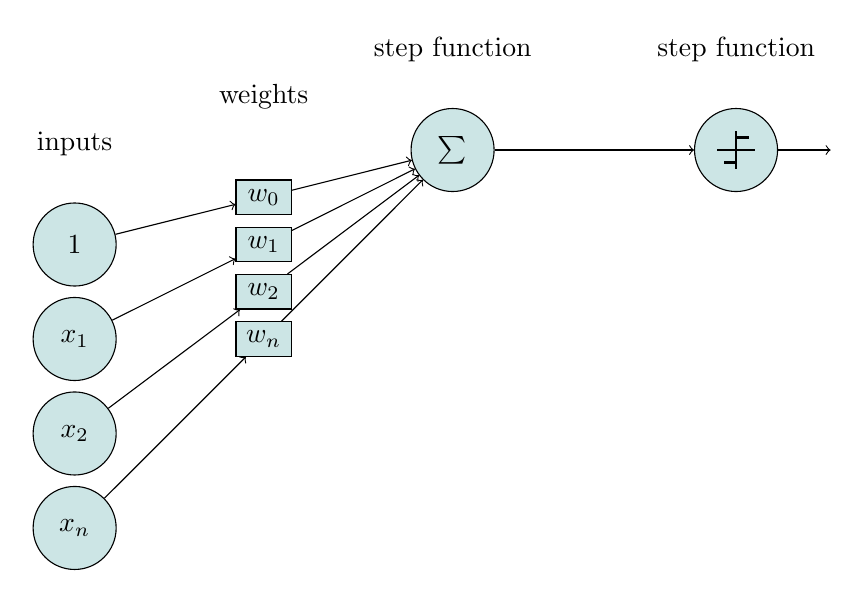
\begin{tikzpicture}[scale=1.2]
    \foreach \h [count=\hi ] in {$x_n$,$x_2$,$x_1$,$1$}{%
          \node[input] (f\hi) at (0,\hi*1cm-5 cm) {\h};
        }
    \node[functions] (sum) at (4,0) {$\sum$};
    \foreach \h [count=\hi ] in {$w_n$,$w_2$,$w_1$,$w_0$}{%
          \path (f\hi) -- node[weights] (w\hi) {\h} (sum);
          \draw[->] (f\hi) -- (w\hi);
          \draw[->] (w\hi) -- (sum);
        }        
    \node[functions] (step) at (7,0) {};
       \begin{scope}[xshift=7cm,scale=.75]
         \addsymbol
       \end{scope}
    \draw[->] (sum) -- (step);
    \draw[->] (step) -- ++(1,0);
    % Labels
    \node[above=1cm]  at (f4) {inputs};
    \node[above=1cm] at (w4) {weights};
    \node[above=1cm] at (step) {step function};
    \node[above=1cm] at (sum) {step function};
    \end{tikzpicture}